\documentclass[11pt, a4paper, onecolumn, oneside]{report}


\usepackage[top=1in, right=1in, bottom=1in, left=1in]{geometry}
\usepackage{xcolor}
\usepackage{graphicx}
\usepackage{cleveref}

\usepackage{minted}
\usemintedstyle{tango}
%interactive references in pdf (slower compilation times)
\usepackage{hyperref}
\hypersetup{
    colorlinks=false,
}

% Stop chapters from starting new pages
% \usepackage{etoolbox}
% \makeatletter
% \patchcmd{\chapter}{\if@openright\cleardoublepage\else\clearpage\fi}{}{}{}
% \makeatother


\title{FLAME GPU Technical Report and User Guide}
\author{Paul Richmond}
\date{\today}
% \date{}

% todo List:
% @todo change author to Paul / FLAME GPU contirbutors
% @todo Create nice title page
% @todo improve document formatting
% @todo better labels (meaningful rather than old section numbers)
% @todo use lstlistings with custom highlighting rules to replace slow minted compilation
% @todo Complete section on using Makefile
% @todo Complete section(s) on graph based communication
% @todo complete section on staticGraph data structure
% @todo describe instrumentation #defines
% @todo add details of host agent creation in init/step fns

\begin{document}

\maketitle

\tableofcontents
% \listoffigures
% \listoftables
% \clearpage

\chapter{Introduction}
\label{ch:1}
Agent Based Modelling is a technique for the computational simulation of complex interacting systems through the specification of the behaviour of a number of autonomous individuals acting simultaneously.
This is a bottom up approach, in contrast with the top down one of modelling the behaviour of the whole system through dynamic mathematical equations. The focus on individuals is considerably more computationally demanding, but provides a natural and flexible environment for studying systems demonstrating emergent behaviour.
Despite the obvious parallelism, traditionally frameworks for ABM fail to exploit this and are often based on highly serialised algorithms for manipulating mobile discrete agents.
Such an approach has serious implications, placing stringent limitations on both the scale of models and the speed at which they may be simulated.
The purpose of the FLAME GPU framework is to address the limitations of previous agent modelling software by targeting the high performance GPU architecture.
The framework is designed with parallelism in mind and as such allows agent models to scale to massive sizes and ensures simulations run within reasonable time constrains.
In addition to this visualisation is easily achievable as simulation data is held entirely within GPU memory where it can be rendered directly.



\section{High Level Overview of FLAME GPU}
\label{sec:11}

Technically the FLAME GPU framework is not a simulator, it is instead a template based simulation environment that maps formal descriptions of agents into simulation code.
The representation of an agent is based on the concept of a communicating X-Machine (which is an extension to the Finite State Machine which includes memory).
Whilst the X-Machine has very formal definition X-Machine agents can be thought of a state machines which are able to communicate via messages which are stored in a globally accessible message lists.
Agent functionality is exposed as a set of state transition functions which move agents from one internal state to another.
Upon changing state, agents update their internal memory through the influence of messages which may be either used as input (by iterating message lists) or as output (where information may be passed to the message lists for other agents to read).
FLAME GPU uses agent function scripting for this purpose where script is defined in a number of \emph{Agent Function Files}.
Simulation models are specified using a format called X-Machine Mark-up Language (\emph{XMML}) which is XML syntax with Schemas governing the content.
A typically XMML model file consists of a definition of a number of X-Machine agents (including state and memory information as well as a set of agent transition functions), a number of message types (each of which has a globally accessible message list) and a set of simulation layers which define the execution order of agent functions (which constitutes a single simulation iteration).
Throughout a simulation, agent data is persistent however message information (and in particular message lists) is persistent only over the lifecycle of a single iteration.
This allows a mechanism for agents to iteratively interact in a way which allows emergent global group behaviour.

The process of generating a FLAME GPU simulation is described by the 1.
The use of XML schemas forms a large part of the process where polymorphic like extension allows a base schema specification to be extended with a number of GPU specific elements.
Given an XMML model definition, template driven code generation is achieved through Extensible Stylesheet Transformations (XSLT).
XSLT is a flexible functional language based on XML (validated itself using a W3C specified Schema) and is suitable for the translation of XML documents into other document formats using a number of compliant processors (although the FLAME GPU SDK provides its own).
Through the specification of a number of \emph{XSLT Simulation Templates} a \emph{Dynamic Simulation API} is generated which links with the \emph{Agent Function Files} to generate a simulation program.

\begin{figure}[ht]
    \centering
    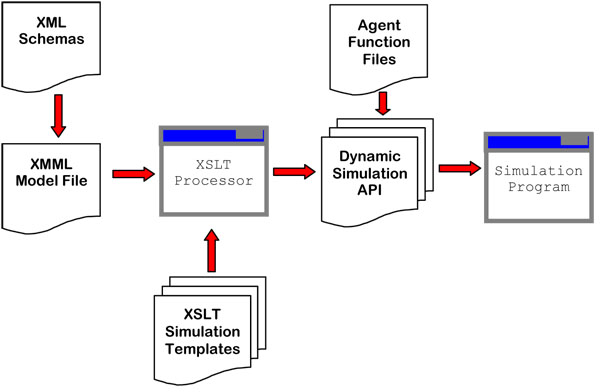
\includegraphics[width=0.70\textwidth]{img/figure1}
    \caption{FLAME GPU Modelling and Simulation Processes}
    \label{fig:modelling-and-simulation-process}
\end{figure} 

\section{Purpose of This Document}
\label{sec:12}

The purpose of this document is to describe the functional parts which make up a FLAME GPU simulation as well as providing guidance on how to use the FLAME GPU SDK.
\Cref{ch:2} describes in detail the syntax and format of the XMML Model file.
\Cref{ch:3} describes the syntax of use of agent function scripts and how to use the dynamic simulation API and \Cref{ch:4} describes how to generate simulation code and run simulations from within the Visual Studio IDE.
This document does not act as a review of background material relating to GPU agent modelling, nor does it provide details on FLAME GPUs implementation or descriptions of the FLAME GPU examples.
For more in depth background material on agent based simulation on the GPU, the reader is directed towards the following document;

\begin{quote}
\emph{Richmond Paul, Walker Dawn, Coakley Simon, Romano Daniela (2010), "High Performance Cellular Level Agent-based Simulation with FLAME for the GPU", Briefings in Bioinformatics, 11(3), pages 334-47.}
\end{quote}

For details on the implementation including algorithms and techniques the reader is directed towards the following publication;

\begin{quote}
\emph{Richmond Paul (2011), "Template Driven Agent Based Modelling and Simulation with CUDA", GPU Computing Gems Emerald Edition (Wen-mei Hwu Editor), Morgan Kaufmann, March 2011, ISBN: 978-0-12-384988-5}

\emph{Richmond Paul, Coakley Simon, Romano Daniela (2009), "A High Performance Agent Based Modelling Framework on Graphics Card Hardware with CUDA", Proc. of 8th Int. Conf. on Autonomous Agents and Multi-Agent Systems (AAMAS 2009), May, 10--15, 2009, Budapest, Hungary}
\end{quote}

Some examples of FLAME GPU models are described in the following publications;

\begin{quote}
\emph{Richmond Paul, Coakley Simon, Romano Daniela (2009), "Cellular Level Agent Based Modelling on the Graphics Processing Unit", Proc. of HiBi09 - High Performance Computational Systems Biology, 14-16 October 2009,Trento, Italy (additional detail in the BiB paper)}

\emph{Karmakharm Twin, Richmond Paul, Romano Daniela (2010), " Agent-based Large Scale Simulation of Pedestrians With Adaptive Realistic Navigation Vector Fields", To appear in Proc. of Theory and Practice of Computer Graphics (TPCG) 2010, 6-8th September 2010, Sheffield, UK}
\end{quote}


\chapter{FLAMEGPU Model Specification}
\label{ch:2}
\section{Introduction}
\label{sec:21}

FLAME GPU models are specified using XML format within an XMML document.
The syntax of the model file is governed by two XML Schemas, an abstract base Schema describes the syntax of a basic XMML agent model (compatible with HPC and CPU versions of the FLAME framework) and a concrete GPU Schema extension this to add various bits of additional model information.
Within this chapter the XML namespace (xmlns) gpu is used to qualify the XML elements which extend the basic Schema representation.
A high level overview of a an XMML model file is described below with various sections within this chapter describing each part in more detail.


\begin{minted}[fontsize=\small,breaklines]{XML}
<gpu:xmodel
    xmlns:gpu="http://www.dcs.shef.ac.uk/\textasciitilde{}paul/XMMLGPU"
    xmlns="http://www.dcs.shef.ac.uk/\textasciitilde{}paul/XMML">
    <name>Model Name</name>    <!-- optional -->
    <gpu:environment>...</gpu:environment>
    <xagents>...</xagents>
    <messages>...</messages>
    <layers>...</layers>
</gpu:xmodel>
\end{minted}

\section{The Environment}
\label{sec:22}


The environment element is used to hold global information which relates to the simulation.
This information includes, zero or more constant, or global, variables (which are constant for all agents over the period of either the simulation or single simulation iteration), a single non optional function file containing agent function script (see \Cref{ch:3}) and an optional number of initialisation, step and exit functions.

\begin{minted}[fontsize=\small,breaklines]{XML}
<gpu:environment>
    <gpu:constants>...</gpu:constants>            <!-- optional -->
    <gpu:functionFiles>...</gpu:functionFiles>    <!-- not optional -->
    <gpu:initFunctions>...</gpu:initFunctions>    <!-- optional -->
    <gpu:stepFunctions>...</gpu:stepFunctions>    <!-- optional -->
    <gpu:endFunctions>...</gpu:endFunctions>      <!-- optional -->
</gpu:environment>
\end{minted}

\subsection{Simulation Constants (Global Variables)}
\label{sec:221}

Simulation constants are defined as (global) variables and may be of type int, float or double (on GPU hardware with double support i.e. CUDA Compute capability 2.0 or beyond).
Constant variables must each have a unique name which is used to reference them within simulation code and can have an optional static array length (of size greater than 0).
The description element arrayLength element and defaultValue element are all optional.
The below code shows the specification of two constant variables: the first represents a single \mintinline[fontsize=\small]{c}{int} constant (with a default value of $1$), the second indicates an \mintinline[fontsize=\small]{c}{int} array of length 5.
Simulation constants can be set either as default values as show below, within the initial agent XML file (see \cref{271}) or at run-time are described in \cref{sec:39}. Values set in initial XML values will overwrite a default value and values which are set at runtime will overwrite values set in initial agent XML files.

\begin{minted}[fontsize=\small,breaklines]{XML}
<gpu:constants>
    <gpu:variable>
        <type>int</type>
        <name>const_variable</name>
        <description>none</description>
        <defaultValue>1</defaultValue>
    </gpu:variable>
    <gpu:variable>
        <type>int</type>
        <name>const_array_variable</name>
        <description>none</description>
        <arrayLength>5</arrayLength>
    </gpu:variable>
</gpu:constants>
\end{minted}

\subsection{Function Files}
\label{sec:222}


The functionFiles element is not optional and must contain a single file element which defines the name of a source code file which holds the scripted agent functions.
More details on the format of the function file are given in \Cref{ch:3}.
The example below shows the correct XML format for a function file named \mintinline[fontsize=\small]{text}{functions.c}.

\begin{minted}[fontsize=\small,breaklines]{XML}
<gpu:functionFiles>
    <file>functions.c</file>
</gpu:functionFiles>
\end{minted}

\subsection{Initialisation Functions}
\label{sec:223}


Initialisation functions are user defined functions which can be used to set constant global variables. 
Any initialisation functions defined within the initFunctions element are called a single time by the automatically generated simulation code in the order that they appear during the initialisation of the simulation. 
If an initFunctions element is specified there must be at least a single initFunction child element with a unique name. 
\Cref{sec:391} demonstrates how to specify initialisation functions within a function file.

\begin{minted}[fontsize=\small,breaklines]{XML}
<gpu:initFunctions>
    <gpu:initFunction>
        <gpu:name>initConstants</gpu:name>
    </gpu:initFunction>
</gpu:initFunctions>
\end{minted}


\subsection{Step Functions}
\label{sec:stepFunc}

Step functions are similarly defined to initialisation functions, requiring at least a single stepFunction child element if the stepFunctions element is defined. These functions are called at the end of each iteration step, i.e. after all the layers, as defined in section \ref{sec:26}, are executed each step. Example uses of this function are to calculate agent averages during the iteration step or sort functions.

\begin{minted}[fontsize=\small,breaklines]{XML}
<gpu:stepFunctions>
    <gpu:stepFunction>
        <gpu:name>some_step_func</gpu:name>
    </gpu:stepFunction>
</gpu:stepFunctions>
\end{minted}

\subsection{Exit Functions}
\label{sec:exitFunc}

Exit functions are again like the other function types defined above, requiring at least a single exitFunction child element if the exitFunctions element is defined. These functions are called at the end of the whole simulation. An example use of this function would be to calculate final averages of agent variables or print out final values.

\begin{minted}[fontsize=\small,breaklines]{XML}
<gpu:exitFunctions>
    <gpu:exitFunction>
        <gpu:name>some_exit_func</gpu:name>
    </gpu:exitFunction>
</gpu:exitFunctions>
\end{minted}


\section{Defining an X-Machine Agent}
\label{sec:23}


A XMML model file must contain a single xagents element which in turn must define at least a single xagent.
An xagent is an agent representation of an X-Machine and consists of a name, optional description, an internal memory set ($M$ in the formal definition), a set of agent functions (or next state partial functions, $F$, in the formal definition) and a set of states ($Q$ in the formal definition).
In addition to this FLAMEGPU requires two additional pieces of information (which are not required in the original XMML specification), a type and a \mintinline[fontsize=\small]{c}{bufferSize}.
The type element refers to the type of agent with respect to its relation with its spatial environment.
An agent type can be either discrete or continuous, discrete agents occupy non mobile 2D discrete spatial partitions (cellular automaton) where as continuous agents are assumed to occupy a continuous space environment (although in reality they may in fact be non spatial more abstract agents).
As all memory is pre-allocated on the GPU a \mintinline[fontsize=\small]{c}{bufferSize} is required to represent the largest possible size of the agent population.
That is the maximum number of x-machine agent instances of the format described by the XMML model.
There is no performance disadvantage to using a large \mintinline[fontsize=\small]{c}{bufferSize} however it is the user's responsibility to ensure that the GPU contains enough memory to support large populations of agents.
It is recommended that the bufferSize always be a power of two number (i.e.
$1024$, $2048$, $4096$, $16384$, etc) as it will most likely be rounded to one during simulation.
For discrete agents the bufferSize is currently limited to only power of 2 numbers which have squarely divisible dimensions (i.e. the square of the bufferSize must be a whole number).
If at any point in the simulation exceeds the stated bufferSize then the user will be warned at the simulation will exit.
Each expandable aspect of an XMML agent representation in the below example is discussed within this section with the exception of agent functions, which due to their dependence of the definition of messages, are discussed later in \cref{sec:25}.

\begin{minted}[fontsize=\small,breaklines]{XML}
<xagents>
    <gpu:xagent>
    <name>AgentName</name>
        <description>optional description of the agent</description>
        <memory>...</memory>
        <functions>...</functions>
        <states>...</states>
        <gpu:type>continuous</gpu:type>
        <gpu:bufferSize>1024</gpu:bufferSize>
    </gpu:xagent>
    <gpu:xagent>
        <!-- ... -->
    </gpu:xagent>
</xagents>
\end{minted}


\subsection{Agent Memory}
\label{sec:231}


Agent memory consists of a number of variables (at least one) which are use to hold information.
An agent variable must have a unique name and may be of type \mintinline[fontsize=\small]{c}{int}, \mintinline[fontsize=\small]{c}{float} or \mintinline[fontsize=\small]{c}{double} (CUDA compute capability 1.3 or beyond).
Default values are always $0$ unless a value is specified within the XML input states file.
There are no specified limits on the maximum number of agent variables however the performance tips noted in \cref{sec:47} should be taken into account.
Agent memory can also be defined as static sized array. For performance use sizes that are a multiple of 2(?)
Below shows an example of agent memory containing four agent variables representing an agent identifier, two positional values and a list of numbers.

\begin{minted}[fontsize=\small,breaklines]{XML}
<memory>
    <gpu:variable>
        <type>int</type>
        <name>id</name>
        <description>variable description</description>
    </gpu:variable>
    <gpu:variable>
        <type>float</type>
        <name>x</name>
    </gpu:variable>
    <gpu:variable>
        <type>float</type>
        <name>y</name>
    </gpu:variable>
    <gpu:variable>
        <type>float</type>
        <name>nums</name>
        <arrayLength>64</arrayLength>
    </gpu:variable>
</memory>
\end{minted}


\subsection{Agent States}
\label{sec:232}

Agent states are defined as a list of state elements ($Q$ in the X-Machine formal definition) with a unique and non optional name.
As simulations within FLAMEGPU can continue indefinitely (or for a fixed number of iterations), terminal states ($T$ in the formal definition) are not defined.
The initial state ($q_{0}$) must however be defined within the initialState element and must correspond with an existing and unique state name from the list of states above it.

\begin{minted}[fontsize=\small,breaklines]{XML}
<states>
    <gpu:state>
        <name>state1</name>
    </gpu:state>
    <gpu:state>
        <name>state2</name>
    </gpu:state>
    <initialState>state1</initialState>
</states>
\end{minted}

\section{Defining Messages}
\label{sec:24}


Messages represent the information which is communicated between agents.
An element messages contains a list of at least one message which defines a non optional name an optional description of the message, a list of variables, a partitioning type and a \mintinline[fontsize=\small]{c}{bufferSize}.
The \mintinline[fontsize=\small]{c}{bufferSize} element is used in the same way that a bufferSize is used to define an X-Machine agent, i.e. the maximum number of this message type which may exist within the simulation at one time.
The partitioning type may be one of three currently defined message partition schemes, non partitioned (\mintinline[fontsize=\small]{c}{partitioningNone}), discrete 2D space partitioning (\mintinline[fontsize=\small]{c}{partitioningDiscrete}) or 2D/3D spatially partitioned space (\mintinline[fontsize=\small]{c}{partitioningSpatial}).
Message partition schemes are used to ensure that the most optimal cycling of messages occurs within agent functions. The use of the partitioning techniques is described within this section, as are message variables.

\begin{minted}[fontsize=\small,breaklines]{XML}
<messages>
    <gpu:message>
        <name>message_name</name>
        <description>optional message description</description>
        <variables>...</variables>
        ...<partitioningType/>... <!-- replace with a partitioning type -->
        <gpu:bufferSize>1024</gpu:bufferSize>
    </gpu:message>
    <gpu:message>...</gpu:message>
</messages>
\end{minted}

\subsection{Message Variables}
\label{sec:241}


The message variables element consists of a number of variables (at least one) which are use to hold communication information.
A variable must have a unique name and may be of type \mintinline[fontsize=\small]{c}{int}, \mintinline[fontsize=\small]{c}{float} or \mintinline[fontsize=\small]{c}{double} (CUDA Compute capability 2.0 or beyond).
As with agent variables message variables only supports the use of single memory values (i.e. no static or dynamic arrays).
Likewise there are no specified limits on the maximum number of message variables however increased message size will have a negative effect on performance in all partitioning cases (and in particular when non partitioned messages are used).
The format of message variable specification shown below is identical to that of agent memory.
The only exception is the requirement of certain variable names which are required by certain partitioning types.
Non partitioned messages have no requirement for specific variables.
Discrete partitioning requires two \mintinline[fontsize=\small]{c}{int} type variables of name \mintinline[fontsize=\small]{c}{x} and \mintinline[fontsize=\small]{c}{y}.
Spatial partitioning requires three \mintinline[fontsize=\small]{c}{float} (or \mintinline[fontsize=\small]{c}{double}) type variables named \mintinline[fontsize=\small]{c}{x}, \mintinline[fontsize=\small]{c}{y} and \mintinline[fontsize=\small]{c}{z}.
The example below shows an example of message memory containing two message variables named id and message\_variable.


\begin{minted}[fontsize=\small,breaklines]{XML}
<variables>
    <gpu:variable>
        <type>int</type>
        <name>id</name>
        <description>variable description</description>
    </gpu:variable>
    <gpu:variable>
        <type>float</type>
        <name>message_variable</name>
    </gpu:variable>
</variables>
\end{minted}

\subsection{Non partitioned Messages}
\label{sec:242}

None partitioned messages do not use any filtering mechanism to reduce the number of messages which will be iterated by agent functions which use the message as input.
None partitioned messages therefore require a brute force or $O(n^{2})$ message iteration loop wherever the message list is iterated.
As non partitioned messages do not require any message variables with location information the partition type is particularly suitable for communication between non spatial or more abstract agents.
Brute force iteration is obviously reasonably computationally expensive, however non partitioned message iteration requires very little overhead (or setup) and as a result for small numbers of messages it can be more efficient than either limited range technique.
There is no strict rule governing performance and different GPU hardware will produce different results depending on it capability.
It is therefore left to the user to experiment with different message partitioning types within a simulation.
The example below shows the format of the partitioningNone element tag.

\begin{minted}[fontsize=\small,breaklines]{XML}
<gpu:partitioningNone/>
\end{minted}

\subsection{Discrete Partitioned Messages}
\label{sec:243}

Discrete partitioned messages are messages which may only originate from non mobile discrete agents (cellular automaton).
A discrete partitioning message scheme requires the specification of a radius which indicates the range (in in 2D discrete space) which a message iteration will extend to.
A radius value of 0 indicates that only a single message will be returned from message iteration.
A value of greater than 0 indicates that message iteration will loop through ±radius in both the \mintinline[fontsize=\small]{c}{x} and a \mintinline[fontsize=\small]{c}{y} dimension (e.g.
a range of $1$ will iterate $3x3=9$ messages, a range of $2$ will iterate $5x5=25$).
In addition to this the agent memory is expected to contain x and y variables of type \mintinline[fontsize=\small]{c}{int}.
As with discrete agents it is important to ensure that messages using discrete partitioning use only supported buffer sizes (power of $2$ and squarely divisible). The width and height of the discrete message space is then defined as the square of the bufferSize value.

\begin{minted}[fontsize=\small,breaklines]{XML}
<gpu:partitioningDiscrete>
    <gpu:radius>1</gpu:radius>
</gpu:partitioningDiscrete>
\end{minted}

\subsection{Spatially Partitioned Messages}
\label{sec:244}

Spatially partitioned messages are messages which originate from continuous spaced agents in either a 3D environment (i.e. agents with \mintinline[fontsize=\small]{c}{x}, \mintinline[fontsize=\small]{c}{y} and \mintinline[fontsize=\small]{c}{z} variables).
A spatially partitioned message scheme requires the specification of both a radius and a set of environment bounds.
The radius represents the range in which message iteration will extend to (from its originating point).
The environment bounds represent the size of the space which massages may exist within.
If a message falls outside of the environment bounds then it will be bound to the nearest possible location within it.
The space within the defined bounds is partitioned according to the radius with a total of P partitions in each dimension, where for each dimension;

$P = ceiling((max\_bound - min\_bound) / radius)$

The partitions dimensions are then used to construct a partition boundary matrix (an example of use within message iteration is provided in \cref{sec:352}) which holds the indices of messages within each area of partitioned space.
Spatially partitioned message iteration can then iterate a varying number of messages from a fixed number of adjacent partitions in partition space to ensure each message within the specified radius has been considered.
The following example defines a spatial partition in three dimensions.
For continuously spaced agents in 2D space $P$ should be equal to $1$ and therefore a \mintinline[fontsize=\small]{text}{zmin} of $0$ would require a \mintinline[fontsize=\small]{text}{zmax} value equal to radius (even in this case a message variable with name \mintinline[fontsize=\small]{c}{z} is still required).

\begin{minted}[fontsize=\small,breaklines]{XML}
<gpu:partitioningSpatial>
    <gpu:radius>1</gpu:radius>
    <gpu:xmin>0</gpu:xmin>
    <gpu:xmax>10</gpu:xmax>
    <gpu:ymin>0</gpu:ymin>
    <gpu:ymax>10</gpu:ymax>
    <gpu:zmin>0</gpu:zmin>
    <gpu:zmax>10</gpu:zmax>
</gpu:partitioningSpatial>
\end{minted}

% \subsection{Graph-Based Communication Messages}
% \label{ssec:graph-comm-xml}
% \textbf{@todo}


\section{Defining an Agent function}
\label{sec:25}


An optional list of agent functions is described within an X-Machine agent representation and must contain a list of at least a single agent function element.
In turn, a function must contain a non optional name, and optional description, a current state, next state, an optional single message input, and optional single message output, an optional single agent output, an optional global function condition, an optional function condition, a reallocation flag and a random number generator flag.
The current state is defined within the currentState element and is used to filter the agent function by only applying it to agents in the specified state.
After completing the agent function agents then move into the state specified within the nextState element.
Both the current and \mintinline[fontsize=\small]{text}{nextState} values are required to have values which exist as a state/name within the state list (states) definition.
The reallocate element is used as an optional flag to indicate the possibility that an agent performing the agent function may die as a result (and hence require removing from the agent population).
By default this value is assumed true however if a value of false is specified then the processes for removing dead agents will not be executed even if an agent indicates it has died (see agent function definitions in \cref{sec:33}).
The RNG element represents a flag to indicate the requirement of random number generation within the agent function.
If this value is true then an additional parameter (demonstrated in \cref{sec:37}) is passed to the agent function which holds a number of seeds used for parallel random number generation.


\begin{minted}[fontsize=\small,breaklines]{XML}
<functions>
    <gpu:function>
        <name>func_name</name>
        <description>function description</description>
        <currentState>state1</currentState>
        <nextState>state2</nextState>
        <inputs>...</inputs>                           <!-- optional -->
        <outputs>...</outputs>                         <!-- optional -->
        <xagentOutputs></xagentOutputs>                <!-- optional -->
        <gpu:globalCondition>...</gpu:globalCondition> <!-- optional -->
        <condition>...</condition>                     <!-- optional -->
        <gpu:reallocate>true</gpu:reallocate>          <!-- optional -->
        <gpu:RNG>true</gpu:RNG>                        <!-- optional -->
    </gpu:function>
</functions>
\end{minted}


\subsection{Agent Function Message Inputs}
\label{sec:251}


An agent function message input indicates that the agent function will iterate the list of messages with a name equal to that specified by the non optional messageName element.
It is therefore required that the messageName element refers to an existing message/name defined within the XMML document.
In addition to this an agent function cannot iterate a list of messages without specifying that it is an input within the XMML model file (message iteration functions are parameterised to prevent this).

\begin{minted}[fontsize=\small,breaklines]{XML}
<inputs>
    <gpu:input>
        <messageName>message_name</messageName>
    </gpu:input>
</inputs>
\end{minted}

\subsection{Agent Function Message Outputs}
\label{sec:252}

An agent function message output indicates that the agent function will output a message with a name equal to that specified by the non optional messageName element.
The messageName element must therefore refer to an existing message/name defined within the XMML document.
It is not possible for an agent function script to output a message without specifying that it is an output within the XMML model file (message output functions are parameterised to prevent this).
In addition to the messageName element a message output also requires a type.
The type may be either \mintinline[fontsize=\small]{c}{single_message} or \mintinline[fontsize=\small]{c}{optional_message}, where \mintinline[fontsize=\small]{c}{single_message} indicates that every agent performing the function outputs exactly one message and \mintinline[fontsize=\small]{c}{optional_message} indicates that agent's performing the function may either output a single message or no message.
The type of messages which can be output by discrete agents are not restricted however continuous type agents can only output messages which do not use discrete message partitioning (e.g.
no partitioning or spatial partitioning).
The example below shows a message output using \mintinline[fontsize=\small]{c}{single_message} type.
This will assume every agent outputs a message, if the functions script fails to output a message for every agent a message with default values (of $0$) will be created instead.

\begin{minted}[fontsize=\small,breaklines]{XML}
<outputs>
    <gpu:output>
        <messageName>message_name</messageName>
        <gpu:type>single_message</gpu:type>
    </gpu:output>
</outputs>
\end{minted}

\subsection{Agent Function X-Agent Outputs}
\label{sec:253}

An agent function xagentOutput indicates that the agent function will output an agent with a name equal to that specified by the non optional xagentName element.
This differs slightly from the formal definition of an x-machine which does not explicitly define a technique for the creation of new agents but adds functionality required for dynamically changing population sizes during simulation runtime.
The xagentName element belonging to an xagentOutput element must refer to an existing agent/name defined within the XMML document.
It is not possible for an agent function script to output a agent without specifying that it is an xagntOutput within the XMML model file (agent output functions are parameterised to prevent this).
In addition to the xagentName element a message output also requires a state.
The state represents the state from the list of state elements belonging to the specified agent\textbackslash{}name that the new agent should be in after it has been created.
Only continuous type agents are allowed to output new agents (which must also be of type continuous).
The creation of new discrete agents is not permitted under any circumstance.
An \mintinline[fontsize=\small]{c}{xagentOutput} does not require a type (as is the case with a message output) and any agent function outputting an agent is assumed to be optional.
I.e. each agent performing the function may output either one or zero agents.

\begin{minted}[fontsize=\small,breaklines]{XML}
<xagentOutputs>
    <gpu:xagentOutput>
        <xagentName>agent_name</xagentName>
        <state>state1</state>
    </gpu:xagentOutput>
</xagentOutputs>
\end{minted}

\subsection{Function Conditions}
\label{sec:254}

An agent function condition indicates that the agent function should only be applied to agents which meet the defined condition (and in the correct state specified by \mintinline[fontsize=\small]{c}{currentState}).
Each function condition consists of three parts a left hand side statement (\mintinline[fontsize=\small]{text}{lhs}), an operator and a right hand side statement (\mintinline[fontsize=\small]{text}{rhs}).
Both the \mintinline[fontsize=\small]{text}{lhs} and \mintinline[fontsize=\small]{text}{rhs} elements may contain either a agentVariable a value or a recursive condition element.
An agentVariable element must refer to a agent variable defined within the agents list of variable names (i.e.
\mintinline[fontsize=\small]{XML}{gpu:xagent/memory/gpu:variable/name}).
A value element may refer to any numeric value or constant definition (defined within the agent function scripts).
The use of recursive conditions is demonstrated below by embedding a condition within the \mintinline[fontsize=\small]{text}{rhs} element of the top level condition.


\begin{minted}[fontsize=\small,breaklines]{XML}
<condition>
    <lhs>
        <agentVariable>variable_name</agentVariable>
    </lhs>
    <operator>&lt;</operator>
    <rhs>
        <condition>
            <lhs>
                <agentVariable>variable_name2</agentVariable>
            </lhs>
            <operator>+</operator>
            <rhs>
                <value>1</value>
            </rhs>
        </condition>
    </rhs>
</condition>
\end{minted}

In the above example the function condition generates the following pseudo code function guard;

\begin{minted}[fontsize=\small,breaklines]{c}
(variable_name) < ((variable_name2)+(1))
\end{minted}

The condition element may refer to any logical operator.
Care must be taken when using angled brackets which in standard form will cause the XML syntax to become invalid.
Rather than the left hand bracket (less than) the correct xml syntax of 
\mintinline[fontsize=\small]{text}{&lt;} should be used.
Likewise the right hand bracket (greater than) should be replaced with 
\mintinline[fontsize=\small]{text}{&gt;}.


\subsection{Global Function Conditions}
\label{sec:255}


An agent global function condition is similar to an agent function in its syntax however it acts as a global switch to determine if the function should be applied to either \emph{all} or \emph{none} of the agents (within the correct state specified by \mintinline[fontsize=\small]{text}{currentState}).
In the case of every agent evaluating the global function condition to true (or to the value specified by the \mintinline[fontsize=\small]{text}{mustEvaluateTo} element) the agent function is applied to \emph{all} of the agents.
In the case that any of the agents evaluate the global function condition to false (or to the logical opposite of the value specified by the \mintinline[fontsize=\small]{text}{mustEvaluateTo} element) then the agent function will be applied to \emph{none} of the agents.
As with an agent function condition a globalCondition consists of a left hand side statement (\mintinline[fontsize=\small]{text}{lhs}), an operator and a right hand side statement (\mintinline[fontsize=\small]{text}{rhs}).
The syntax of the left hand side statement (\mintinline[fontsize=\small]{text}{lhs}), the operator and the right hand side statement (\mintinline[fontsize=\small]{text}{rhs}) is the same as with an agent function condition and may use recursion to generate a complex conditional statement.
The maxItterations element is used to limit the number of times a function guarded by the global condition can be avoided (or evaluated as the logical opposite of the value specified by the \mintinline[fontsize=\small]{text}{mustEvaluateTo} element).
For example, the definition at the end of this section, resulting in the following pseudo code condition;

\begin{minted}[fontsize=\small,breaklines]{c}
(((movement) < (0.25)) == true)
\end{minted}
May be evaluated as false up to $200$ times (i.e. in $200$ separate simulation iterations) before the global condition will be ignored and the function is applied to every agent.
Following maximum number of iterations being reached the iteration count is reset once the agent function has been applied.

\begin{minted}[fontsize=\small,breaklines]{XML}
<gpu:globalCondition>
    <lhs>
        <agentVariable>movement</agentVariable>
    </lhs>
    <operator>&lt;</operator>
    <rhs>
        <value>0.25</value>
    </rhs>
    <gpu:maxItterations>200</gpu:maxItterations>
    <gpu:mustEvaluateTo>true</gpu:mustEvaluateTo>
</gpu:globalCondition>
\end{minted}


\section{Function Layers}
\label{sec:26}

Function layers represent the control flow of the simulation processes.
The sequence of layers defines the sequential order in which agent functions are executed.
Complete execution of every layer of agent functions represents a single simulation iteration which may be repeated any number of times.
Syntatically within the model definition a single layers element must contain at least one (or more) layer element.
Each layer element may contain at least one (or more) \mintinline[fontsize=\small]{XML}{gpu}:layerFunction element which defines only a name which must relate to a function name specified within a corresponding \mintinline[fontsize=\small]{text}{xagents/gpu:xagent/functions/gpu:function/name}.
Within a given layer, the order of execution of layer functions should not be assumed to be sequential (although in the current version of the software it is, future versions will execute functions within the same layer in parallel).
For the same reason functions within the same layer should not have any communication or internal dependencies (for example via message communications or execution order dependency) in which case they should instead be represented within separate layers which guarantee execution order and global synchronisation between the functions.
The below example demonstrates the syntax of specifying a simulation consisting of three agent functions.
There are no dependencies between \mintinline[fontsize=\small]{text}{function1} and \mintinline[fontsize=\small]{text}{function2} which in this case can be thought of as being functions from two different agents definitions with no shared message input or output.


\begin{minted}[fontsize=\small,breaklines]{XML}
<layers>
    <layer>
        <gpu:layerFunction>
            <name>function1</name>
        </gpu:layerFunction>
        <gpu:layerFunction>
            <name>function2</name>
        </gpu:layerFunction>
    </layer>
    <layer>
        <gpu:layerFunction>
            <name>function3</name>
        </gpu:layerFunction>
    </layer>
</layers>
\end{minted}


\section{Initial XML Agent Data}
\label{sec:27}


The initial agent data information is stored in an XML file which is passed to the simulator as a parameter before running the simulation.
Within this initial agent data XML file, a single states element contains a single iteration number (\mintinline[fontsize=\small]{text}{itno}) and any number (including 0) of xagent elements.
The syntax of the xagent element depends on the agent definitions contained within the XMML model definition file.
A name element is always required and must represent an agent name contained within a \mintinline[fontsize=\small]{text}{xgents/gpu:agent/name} element in the XMML model definition.
Following this an element may exist for each of the named agents memory variables (\mintinline[fontsize=\small]{text}{xagents/gpu:agent/memory/gpu:variable/name}).
Each named element is then expected to contain a value of the same type as the agent memory variable defined.
If the initial agent data XML file neglects to specify the value of a variable defined within an agents memory then the value is assumed to be zero.
If an element defines a variable name which does not exist within the XMML model definition then a warning is generated and the value is ignored.
The example below represents a single agent corresponding to the agent definition in \cref{sec:23}.

\begin{minted}[fontsize=\small,breaklines]{XML}
<states>
    <itno>0</itno>
    <xagent>
        <name>AgentName</name>
        <id>1</id>
        <x>21.088</x>
        <y>12.834</y>
        <z>5.367</z>
    </xagent>
    <xagent>...</xagent>
</states>
\end{minted}

Care must be taken in ensuring that the set of initial data for the simulation does not exceed any of the defined bufferSize (i.e. the maximum number of a given type of agents) for any of the agents.
If buffer size is exceeded during initial loading of the initial agent data then the simulation will produce an error.

Another special case to consider is the use of 2D discrete agents where the number of agents within the set of initial agent data must match exactly the bufferSize (which must also be a power of 2) defined within the XMML models agent definition.
Furthermore the simulation will expect to find initial agents stored within the XML file in row wise ascending order.

\subsection{Initial Simulation Constants}
\label{sec:271}

Simulation constants (or global variables) specified within the model file (as described in \cref{sec:229}) can be set within the initial XML agent data within an environment label between the itno and xagent elements. Environment variables should be set within an XML element with a name corresponding to the environment variable name. E.g. An environment variable defined within the model file as;

\begin{minted}[fontsize=\small,breaklines]{XML}
<gpu:constants>
    <gpu:variable>
        <type>int</type>
        <name>my_variable</name>
        <description>none</description>
        <defaultValue>1</defaultValue>
    </gpu:variable>
</gpu:constants>
\end{minted}

Could be defined within an initial XML agents file as follows;

\begin{minted}[fontsize=\small,breaklines]{XML}
<states>
<itno>0</itno>
    <environment>
        <my_variable>2</my_variable>
    </environment>
...
\end{minted}

Note that the value obtained from the initial XML agents file will over-wite any default value.

\chapter{FLAMEGPU Agent Function Scripts and the Simulation API}
\label{ch:3}
\section{Introduction}
\label{sec:31}



Agent function scripts define the behaviour of agents by describing changes to memory and through the iteration and creation of messages and new agents.
The behaviour of the agent function is described from the perspective of a single agent however the simulator will apply in parallel the same agent function code to each agent which is in the correct start state (and meets any of the defined function conditions).
Agent function scripts are defined using a simple C based syntax with the agent function declarations, and more specifically the function arguments dependant on the XMML function definition.
The use of message input and output as well as random number generation will all change the function arguments in a way which is described within this section.
Likewise the simulation API functions for message communication are dependent on the definition of the simulation model contained with the XMML model definition.
A single C source file is required to hold all agent function declarations and must contain an include directive for the file ``\mintinline[fontsize=\small]{text}{header.h}'' which contains model specific agent and message structures.
Agent functions are free to use many features of common C syntax with the following important exceptions; 

\begin{itemize}
\item Globally Defined Variables: i.e. Variables declared outside of any function scope.
    Are not permitted and should instead be defined as global variables within the XMML model file and used as described in \cref{sec:221}.
    Note: The use of pre-processor macro directives for constants is supported and can be freely used without restriction.
\item Include Directives: Are permitted however as agent functions are functions which are ran on the GPU during simulation they may not call non GPU code.
    This implies that including and linking with non CUDA libraries is not supported.
\item External Function Calls: As above external function calls may only be made to CUDA \mintinline[fontsize=\small]{text}{__device__} functions.
    Many common math functions calls such as \mintinline[fontsize=\small]{text}{sin}, \mintinline[fontsize=\small]{text}{cos}, etc.
    are supported via native GPU implementations and can be used in exactly the same way as standard C code.
    Likewise additional ``\mintinline[fontsize=\small]{text}{helper}'' functions can be defined and called from agent functions by prefixing the helper function using the \mintinline[fontsize=\small]{text}{__FLAME_GPU_FUNC__} macro (which signifies it can be run on the GPU device).
\end{itemize}

The following chapter describes the syntax and use of agent function scripts including any arguments which must be passed to the agent or simulation API functions.
As agent functions and simulation API functions are dynamic (and based on the XMML model definition) it is often easier to first define a model and use the technique described within \cref{sec:42} to automatically generate a functions file containing prototype agent function files and API system calls.
Alternatively \cref{sec:38} describes fully the expected argument order for agent function arguments.


\section{Agent and Message Data Structures}
\label{sec:32}

Access to agent and message data within the agent function scripts is provided through the use of agent and message data structures which contain variables matching those defined within the XMML definitions.
For each agent in the simulation a structure is defined within the dynamically generated header.h with the name \mintinline[fontsize=\small]{text}{xmachine_memory_agent_name}, likewise each message defines a structure with the name \mintinline[fontsize=\small]{text}{xmachine_message_message_name}.
In both cases the structures contain a number of private variables prefixed with an underscore (\mintinline[fontsize=\small]{text}{_}) which are used by the API functions and should not be modified directly.
In addition to this the simulation API defines structures of arrays to hold agent and message list information.
Agent lists are named \mintinline[fontsize=\small]{text}{xmachine_memory_agent_name_list} and message lists are named \mintinline[fontsize=\small]{text}{xmachine_message_message_name_list}.
These lists are passed as arguments to agent functions and should only be used in conjunction with the simulation API functions for message iteration and the adding of messages and agents.
List structures should never be accessed directly as doing so will produce undefined behaviour.

\section{A Basic Agent Function (Updating and Agents Memory}
\label{sec:33}


The following example shows a simplistic agent function (named \mintinline[fontsize=\small]{text}{function1}) which has no message input or output and only updates the agents internal memory.
All FLAME GPU agent functions are first prefixed with the macro definition \mintinline[fontsize=\small]{text}{__FLAME_GPU_FUNC__}.
In this basic example the agent function has only a single argument, a pointer to an agent structure of type \mintinline[fontsize=\small]{text}{xmachine_memory_myAgent} called \mintinline[fontsize=\small]{text}{xmemory}..
In the below example the agent name is myAgent and the agent memory contains two variables \mintinline[fontsize=\small]{text}{x} and \mintinline[fontsize=\small]{text}{no_movements} of type \mintinline[fontsize=\small]{text}{float} and \mintinline[fontsize=\small]{text}{int} respectively.
The return type of FLAME GPU functions is always \mintinline[fontsize=\small]{text}{int}.
A return value of anything other than $0$ indicates that the agent has dies and should be removed from the simulation (unless the agent function definition had specifically set the reallocate element value to false in which case any agent deaths will be ignored).


\begin{minted}[fontsize=\small,breaklines]{C}
__FLAME_GPU_FUNC__ int function1(xmachine_memory_myAgent* xmemory)
{
    xmemory->x = xmemory->x += 0.01f;
    xmemory->no_movements += 1;
    return 0;
}
\end{minted}

\section{Use of the Message Output Simulation API}
\label{sec:34}


Within an agent function script message output is possible by using a message output function.
For each message type defined within the XMML model definition the dynamically generated simulation API will create a message output function of the following form; 


\begin{minted}[fontsize=\small,breaklines]{C}
add_message_name_message(message_name_messages, args...);
\end{minted}

Where \mintinline[fontsize=\small]{text}{message_name} refers to the value of the messages name element within the message specification and \mintinline[fontsize=\small]{text}{args} is a list of named arguments which correspond to the message variables (see \cref{sec:241}).
Agent functions may only call a message output function for the message name defined within the function definitions output (see \cref{sec:252}).
This restriction is enforced as message output functions require a pointer to a message list which is passed as an argument to the agent function (\mintinline[fontsize=\small]{text}{xmachine_message_location_list} in the below example).
Agents are only permitted to output a single message per agent function and repeated calls to an add message function will result in previous message information simply being overwritten.
The example below demonstrates an agent function (\mintinline[fontsize=\small]{text}{output_message}) belonging to an agent named myAgent which outputs a message with four variables.
For clarity the message output function prototype (normally found in header.h) is also shown.

\begin{minted}[fontsize=\small,breaklines]{C}
add_location_message(xmachine_message_location_list* location_messages, int id, float x, float y, float z);

__FLAME_GPU_FUNC__ int output_message(xmachine_memory_myAgent* xmemory, xmachine_message_location_list* location_messages)
{
    int id;
    float x, y, z;
    id = xmemory->id;
    x = xmemory->x;
    y = xmemory->y;
    z = xmemory->z;

    add_location_message(location_messages, id, x, y, z);

    return 0;
}
\end{minted}

\section{Use of the Message Input Simulation API}
\label{sec:35}

As with message outputs, iterating message lists (message input) within agent functions is made possible by the use of dynamically generated message API functions.
In general two functions are provided for each named message, a \mintinline[fontsize=\small]{text}{get_first_message_name_message(args...)} and \mintinline[fontsize=\small]{text}{get_next_message_name_message(args...)} the second of which can be used within a while loop until it returns a NULL value indicating the end of the message list.
The arguments of these functions differ slightly depending on the partitioning scheme used by the message.
The following subsections describe these in more detail.
Regardless of the partitioning type a number of important rules must be observed when using the message functions.
Firstly it is essential that message loop complete naturally.
I.e. the \mintinline[fontsize=\small]{text}{get_next_message_name_message} function must be called without breaking from the while loop until the end of the message list is reached.
Secondly agent functions must not directly modify messages returned from the get message functions.
Changing message data directly will result in undefined behaviour and will most likely crash the simulation 


\subsection{Non Partitioned Message Iteration}
\label{sec:351}


For non partitioned messages the dynamically generated message API functions are relatively simple and the arguments which are passed to the API functions are also required by all other message partitioning schemes.
The get first message API function (i.e. \mintinline[fontsize=\small]{text}{get_first_message_name_message}) takes only a single argument which is a pointer to a message list structure (of the form \mintinline[fontsize=\small]{text}{xmachine_message_message_name_list}) which is passed as an argument to the agent function.
The get next message API function (i.e.
\mintinline[fontsize=\small]{text}{get_next_message_name_message}) takes two arguments, the previously returned message and the message list.
The below example shows a complete agent function (\mintinline[fontsize=\small]{text}{input_messages}) demonstrating the iteration of a message list (where the message name location is highlighted within the structure and API names for clarity).
The while loop continues until the get next message API function returns a NULL (or false) value.
In the below example the location message is used to calculate an average position of all the locations specified in the message list.
The agent then updates three of its positional values to move towards the average location (cohesion).

\begin{minted}[fontsize=\small,breaklines]{C}
__FLAME_GPU_FUNC__ int input_messages(xmachine_memory_myAgent* xmemory, xmachine_message_location_list* location_messages)
{
    int count;
    float avg_x, avg_y, agv_z,

    /* Get the first location messages */
    xmachine_message_location* message;
    message = get_first_location_message(location_messages);

    /* Loop through the messages */
    while(message)
    {
        if((message->id != xmemory->id))
        {
            avg_x += message->x;
            avg_y += message->y;
            avg_z += message->z;
            count++;
        }

        /* Move onto next location message */
        message = get_next_location_message(message, location_messages);

    }

    if (count)
    {
        avg_x /= count;
        avg_y /= count;
        avg_z /= count;
    }

    xmemory->x += avg_x * SMALL_NUMBER;
    xmemory->y += avg_y * SMALL_NUMBER;
    xmemory->z += avg_z * SMALL_NUMBER;

    return 0;
}
\end{minted}

\subsection{Spatially Partitioned Message Iteration}
\label{sec:352}

For spatially partitioned messages the dynamically generated message API functions rely on the use of a Partition Boundary Matrix (PBM).
The PBM holds important information which determines which agents are located within the spatially partitioned areas making up the simulation environment.
Wherever a spatially partitioned message is defined as a function input (within the XMML model definition) a PMB argument should directly follow the input message list in the list of agent function arguments.
As with non partitioned messages the first argument of the get first message API function is the input message list.
The second argument is the PBM and the subsequent 3 arguments represent the position which the agent would like to read messages from (which in almost all cases is the agent position).
The get next message API function differs only from the non partitioned example in that the PBM is passed as an additional parameter.
The example below shows the same example as in the previous section but using a spatially partitioned message type (rather than the non partitioned type).
The differences between the function arguments in the previous section are highlighted in red as is the use of a helper function \mintinline[fontsize=\small]{text}{in_range}.
The purpose of the \mintinline[fontsize=\small]{text}{in_range} function is to check the distance between the agent position and the message.
This is important as the messages returned by the get next message function represent any messages within the same or adjacent partitioning cells (to the position specified by the get first message API function).
On average roughly 1/3 of these values will be within the actually range specified by the message definitions range value.


\begin{minted}[fontsize=\small,breaklines]{C}
__FLAME_GPU_FUNC__ int input_messages(xmachine_memory_location* xmemory, xmachine_message_location_list* location_messages, xmachine_message_location_PBM* partition_matrix)
{
    int count;
    float avg_x, avg_y, agv_z,

    /* Get the first location messages */
    xmachine_message_location* location_message;
    message = get_first_location_message(location_messages,
        partition_matrix,
        xmemory->x,
        xmemory->y,
        xmemory->z);
    /* Loop through the messages */
    while(message)
    {
        if (in_range(message, xmemory))
        {
            if((message->id != xmemory->id))
            {
                avg_x += message->x;
                avg_y += message->y;
                avg_z += message->z;
                count++;
            }
        }

        /* Move onto next location message */
        message = get_next_location_message(message,
        location_messages,
        partition_matrix);
    }
    if (count)
    {
        avg_x /= count;
        avg_y /= count;
        avg_z /= count;
    }
    xmemory->x += avg_x * SMALL_NUMBER;
    xmemory->y += avg_y * SMALL_NUMBER;
    xmemory->z += avg_z * SMALL_NUMBER;
    return 0;
}
\end{minted}

\subsection{Discrete Partitioned Message Iteration}
\label{sec:353}


For discretely partitioned messages the dynamically generated message API functions differ from those of non partitioned only in that two additional parameters must be passed to the get first message API function.
The two integer arguments represent the position which the agent would like to read messages from within the cellular environment (as with spatially partitioning this is usually the agent position).
These values of these arguments must therefore be within the width and height of the message space itself (the square of the messages \mintinline[fontsize=\small]{text}{bufferSize}).
In addition to the additional arguments, the discrete message API functions also make use of template parameterisation to distinguish between the type of agent requesting message information.
The template parameters which may be used are either \mintinline[fontsize=\small]{text}{DISCRETE_2D} (as in the example below) or \mintinline[fontsize=\small]{text}{CONTINUOUS}.
This parameterisation is required as underlying implementation of the message API functions differs between the two agent types.
The example below shows an agent function (\mintinline[fontsize=\small]{text}{input_messages}) of a discrete agent (named cell) which iterates a message list (of state messages) to count the number neighbours with a state value of $1$.
The differences between the function arguments in the section describing non partitioned message iteration are highlighted in red as is the function parameterisation.

\begin{minted}[fontsize=\small,breaklines]{C}
__FLAME_GPU_FUNC__ int input_messages(xmachine_memory_cell* xmemory, xmachine_message_state_list* state_messages)
{
    int neighbours = 0;
    xmachine_message_state* state_message;
    message = get_first_state_message<DISCRETE_2D>(state_messages, xmemory->x, xmemory->y);
    
    while(message){
        if (message->state == 1){
            neighbours++;
        }
        message = get_next_state_message<DISCRETE_2D>(message, state_messages);
    }
    xmemory->neighbours = neighbours;
    return 0;
}
\end{minted}

% \subsection{Graph-Based Communication Message Iteration}
% \label{sec:graph-comm-message-iteration}
% \textbf{@todo}


\section{Use of the Agent Output Simulation API}
\label{sec:36}

Within an agent function script agent output is possible by using a message output API function.
For each agent type defined within the XMML model definition the dynamically generated simulation code will create an agent output function of the following form; 
\mintinline[fontsize=\small]{text}{add_agent_name_agent(agent_name_agent, args...);}

Where \mintinline[fontsize=\small]{text}{agent_name} refers to the value of the agents name element within the agent specification and \mintinline[fontsize=\small]{text}{args} is a list of named arguments which correspond to the agents memory variables (see \cref{sec:253}).
Agent functions may only output a single type of agent and are only permitted to output a single agent per agent function.
As with message outputs, repeated calls to an add agent function will result in previous agent information simply being overwritten.
The example below demonstrates an agent function (\mintinline[fontsize=\small]{text}{create_agent}) which outputs a new agent by creating a clone of itself.
For clarity the agent output API function prototype (normally found in \mintinline[fontsize=\small]{text}{header.h}) is also shown.

\begin{minted}[fontsize=\small,breaklines]{C}
add_myAgent_agent(xmachine_memory_myAgent_list* myAgent_agents, int id, float x, float y, float z);

__FLAME_GPU_FUNC__ int output_message(xmachine_memory_myAgent* xmemory, xmachine_memory_myAgent_list* myAgent_agents)
{
    int id;
    float x, y, z;
    id = xmemory->id;
    x = xmemory->x;
    y = xmemory->y;
    z = xmemory->z;
    add_myAgent_agent(myAgent_agents, id, x, y, z);
    return 0;
}
\end{minted}


\section{Using Random Number Generation}
\label{sec:37}


Random number generation is provided via the \mintinline[fontsize=\small]{text}{rnd} API function which uses template parameterisation to distinguish between either discrete (where a parameter value of \mintinline[fontsize=\small]{text}{DISCRETE_2D} should be used) or continuous (where a parameter value of \mintinline[fontsize=\small]{text}{CONTINUOUS} should be used) spaced agents.
If a template parameter value is not specified then the simulation will assume a \mintinline[fontsize=\small]{text}{DISCRETE_2D} value which will work in either case but is more computationally expensive.
The API function has a single argument, a pointer to a \mintinline[fontsize=\small]{text}{RNG_rand48} structure which contains random seeds and is passed to agent functions which specify a true value for the RNG element in the XMML function definition.
The example below shows a simple agent function (with no input or outputs) demonstrating the random number generation to determine if the agent should die.

\begin{minted}[fontsize=\small,breaklines]{C}
#define DEATH_RATE 0.1f

__FLAME_GPU_FUNC__ int kill_agent(xmachine_memory_myAgent* agent, RNG_rand48* rand48)
{
    float random;
    int die;

    die = 0; /* agent does not die */
    random = rnd<CONTINUOUS>(rand48);
    if (random < DEATH_RATE)
        die = 1; /* agent dies */
    
    return die;
}
\end{minted}

\section{Summary of Agent Function Arguments}
\label{sec:38}


Agent functions may use any combination of message input, output, agent output and random number generation resulting in a large number of agent function arguments which are expected to be in a specific and pre defined order.
The following pseudo code demonstrates the order of a function containing all possible arguments.
When specifying an agent function declaration this order must be observed.

\begin{minted}[fontsize=\small,breaklines]{C}
__FLAME_GPU_FUNC__ int function(xmachine_memory_agent_name* agent,
                                xmachine_memory_ agent_name _list* output_agents,
                                xmachine_message_message_name_list* input_messages,
                                xmachine_message_message_name_PBM* input_message_PBM,
                                xmachine_message_message_name_list* output_messages,
                                RNG_rand48* rand48);
\end{minted}

\section{Setting Simulation Constants (Global Variables)}
\label{sec:39}


Simulation constants defined within the environment section of the XMML model definition (or the intial agents state file) may be directly referenced within an agent function using the name specified within the variable definition (see \cref{sec:221}).
It is not possible to set constant variables within an agent function however, the simulation API creates methods for setting simulation constants which may be called either at the start of the simulation (either manually or within an initialisation function) or between simulation iterations (for example as part of an interactive visualisation).
The code below demonstrates the function prototype for setting a simulation constant with the name \mintinline[fontsize=\small]{text}{A_CONSTANT}.


\begin{minted}[fontsize=\small,breaklines]{C}
extern "C" void set\_A\_CONSTANT (float* h\_A\_CONSTANT);
\end{minted}

The function is declared using the extern keyword which allows it to be linked to by externally compiled code such as a visualisation or custom simulation loop.

\subsection{Initialisation Functions}
\label{sec:391}


Any initialisation functions defined within the XMML model file (see \cref{sec:223}) are expected to be declared within an agent function code file and will automatically be called before the first simulation iteration.
The initialisation function declaration should be preceded with a \mintinline[fontsize=\small]{text}{__FLAME_GPU_INIT_FUNC__} macro definition, should have no arguments and should return void.
The below example demonstrated an initialisation function named initConstants which uses the simulation APIs dynamically created constants functions to set a constant named \mintinline[fontsize=\small]{text}{A_CONSTANT}. 

\begin{minted}[fontsize=\small,breaklines]{C}
__FLAME_GPU_INIT_FUNC__ void initConstants()
{
    float const_value = 8.25f;
    set_A_CONSTANT(&const_value);
}
\end{minted}


\subsection{Step Functions}
\label{sec:stepFuncScript}

If a step function was defined in the XMMl model file (section \ref{sec:stepFunc}) then it should be defined in a similar way to the initialisation functions as described above in section \ref{sec:391}. These functions will be called after each iteration step. An example is shown below

\begin{minted}[fontsize=\small,breaklines]{C}
__FLAME_GPU_STEP_FUNC__ void some_step_func()
{
    do_step_operation();
}
\end{minted}


\subsection{Exit Functions}
\label{sec:exitFuncScript}

If an exit function was defined in the XMMl model file (section \ref{sec:endFunc}) then it should be defined in a similar way to the initialisation and step functions as described above. It will be called upon finishing the program. An example is shown below

\begin{minted}[fontsize=\small,breaklines]{C}
__FLAME_GPU_EXIT_FUNC__ void some_exit_func()
{
    calculate_agent_position_average();
    print_to_file();
}
\end{minted}

\section{Instrumentation for timing and population sizes}
\label{sec:TimingAndPop}

It is possible to obtain information of population and timinings of different functions by taking advantage of cuda timing events. Per-iteration and per-function (init/agent/step/exit functions) timing using cuda events, and also the population size for each agent state per iteration printed to stdout.

This instrumentation is enabled with a set of defines. The value must be a positive non-zero integer (i.e. 1) to be enabled.

When enabled, the relevant measures are printed to stdout, which can then later be parsed to produce graphs, etc.

\begin{minted}[fontsize=\small,breaklines]{C}
#define INSTRUMENT_ITERATIONS 1
#define INSTRUMENT_AGENT_FUNCTIONS 1
#define INSTRUMENT_INIT_FUNCTIONS 1
#define INSTRUMENT_STEP_FUNCTIONS 1
#define INSTRUMENT_EXIT_FUNCTIONS 1
#define OUTPUT_POPULATION_PER_ITERATION 1
\end{minted}

will print out, for example
\begin{minted}[fontsize=\small,breaklines]{C}
processing Simulation Step 1
Instrumentation: Circle_outputdata = 0.304128 (ms)
Instrumentation: Circle_inputdata = 16.849920 (ms)
Instrumentation: Circle_move = 0.261120 (ms)
FLAME GPU Step function. Average circle position is (4115.978027, 4139.279785, 512.000000)
Instrumentation: stepFunction = 27.652096 (ms)
agent_Circle_default_count: 1024
Instrumentation: Iteration Time = 46.309376 (ms)
Iteration 1 Saved to XML
\end{minted}

\section{Simulation functions}

These simulation functions are ran independent of agents. More technically they are called on the CPU, but are able to execute GPU functions using the usual CUDA notation. These functions are defined in the dynamically created file \mintinline[fontsize=\small]{text}{simulation.cu}. There are numerous functions which can be called which will be explained in the proceeding sections. These functions can be called during any host/CPU function such as the init, step and end FLAME calls (see section \ref{sec:223} to \ref{sec:endFunc} and \ref{sec:391} to \ref{sec:endFuncScript}).

\subsection{Sort agents}

%function definition
\begin{minted}[fontsize=\small,breaklines]{C}
void sort_agent_default(void (*generate_key_value_pairs)(unsigned int* keys, unsigned int* values, xmachine_memory_agent_list* agents))
\end{minted}

%description of function
This function will sort the agent type called \mintinline[fontsize=\small]{text}{agent} using key-value pairs. The function takes as an argument a function pointer to a GPU \mintinline[fontsize=\small]{text}{__global__} function. This function it points to takes two unsigned int arrays in which it will store the resulting key and value data, and \mintinline[fontsize=\small]{text}{xmachine_memory_agent_list} which contains a structure of arrays of the agent. This type is generated dynamically depending on the agent variables defined in the XML model file (section \ref{sec:231}). For an agent with 2 float variables x and y, it has the following structure:

\begin{minted}[fontsize=\small,breaklines]{C}
struct xmachine_memory_pedestrian_list 
{	
    float x [xmachine_memory_agent_MAX];
    float y [xmachine_memory_agent_MAX];
}
\end{minted}

The value \mintinline[fontsize=\small]{text}{xmachine_memory_agent_MAX} is the and buffer size of number of agents (section \ref{sec:23}). This struct can be accessed to assign agent data to the key and value arrays. The following example is given within a FLAME step function which sorts agents by 1D position

\begin{minted}[fontsize=\small,breaklines]{C}
__global__ void gen_keyval_pairs(unsigned int* keys, unsigned int* values, xmachine_memory_agent_list* agents) {
	int index = (blockIdx.x*blockDim.x) + threadIdx.x;

	//Number of agents
	const int n = xmachine_memory_agent_MAX;

	if (index < n) {
		//set value
		values[index] = index;
		//set key
		keys[index] = agents->x[index];
	}
}

__FLAME_GPU_STEP_FUNC__ void sort_func() {
	
	//Pointer function taking arguments specified within sort_agent_default
	void (*func_ptr)(unsigned int*, unsigned int*, xmachine_memory_agent_list*) = &gen_keyval_pairs;
    
	//sort the key value pairs initialized within argument function
	sort_agent_default(func_ptr);
	
    //Since we run GPU code, make sure all threads are synchronized.
	cudaDeviceSynchronize();
}
\end{minted}

\subsection{Analytic functions}
A dynamically generated reduce is made for all agent variables for each state. Dynamically generated count will only occur for single-values int variables. Reduce sums over a particular variable type for all agents in a state and returns the grand total. Count checks how many values are equal to the given input and returns the quantity that match. These can be called from any \mintinline[fontsize=\small]{text}{__FLAME_GPU__} init, step and end func.Technical: calls thrust reduce or count. 

\begin{minted}[fontsize=\small,breaklines]{C}
reduce_name_state_varName_variable();
count_name_state_varName_variable(int count_value);
\end{minted}



%%%%%%%%%%%%%%%%%%%%%%%%%%%%%%%%%%%%%%%%%%%%%%%%%%%
\chapter{FLAME GPU Simulation and Visualisation}
\label{ch:4}
\section{Introduction}
\label{sec:41}


The processes of building and running a simulation is made easier described within this chapter as are a number of tools and procedures which simplify the simulation code generation and compilation of simulation executables.
In order to use the FLAME GPU SDK it should be placed in a directory which does not contain any spaces (preferably directly within the C: drive or root or root operating system drive).
The host machine must also be running windows with a copy of the .NET runtime (used within the XSLT template processor) and must contain NVIDIA GPU hardware with Compute level 1.0.

\section{Generating a Functions File Template}
\label{sec:42}


\Cref{sec:38} previously described the exact argument order for agent function declarations however in most cases it is sensible to use the provided XSLT template (\mintinline[fontsize=\small]{text}{functions.xslt} located in the \emph{FLAMEGPU/templates} folder within the FLAME GPU SDK) to generate a agent function source file with empty agent function declarations automatically using your XMML model file.
Once this has been generated the agent function scripts can be implemented within the function declarations rather easily.
Care must however be taken in ensuring that if the XMML model file is later modified that the agent function arguments are updated manually where necessary.
Likewise be careful not to overwrite any existing function source file when generating a new one using the XSLT template.
Generation of blank function source files is not incorporated into the visual studio template project and must be manually accomplished.
A .NET based XSLT processor is provided within the FLAME GPU SDK for this purpose (\mintinline[fontsize=\small]{text}{XSLTProcessor.exe} located in the \mintinline[fontsize=\small]{text}{tools} folder) and can be used via the command line as follows (or via the \mintinline[fontsize=\small]{text}{GenerateFunctionsFileTemplate} batch file located in the \mintinline[fontsize=\small]{text}{tools} folder of the FLAME GPU SDK);

\begin{minted}[fontsize=\small,breaklines]{text}
XSLTProcessor.exe XMLModelFile.xml functions.xslt functions.c
\end{minted}

Alternatively any compliant XSLT processor such as Xalan, Unicorn or even Firefox web browser can be used.

\section{FLAME GPU Template Files}
\label{sec:43}


The FLAME GPU SDK contains a number of XSLT templates which are used to generate the dynamic simulation code.
A brief summary of the functionality and contents of each template file is as follows; 

\begin{itemize}
    \item \mintinline[fontsize=\small]{text}{header.xslt} -- This template file generates a header file which contains any agent and message data structures which are common in many of the other dynamically generated simulation source files.
        The template also generates function prototypes for simulation functions and functions which are visible externally within custom C or C++ code.
    \item \mintinline[fontsize=\small]{text}{main.xslt} -- This template file generates a source file which defines the main execution entry point function which is responsible for handling command line options and initialising the GPU device.
    \item \mintinline[fontsize=\small]{text}{io.xslt} -- This template file generates a source file which contains functions for loading initial agent XML data files (see \cref{sec:27}) into the simulation and saving the simulation state back into XML   format.
    \item \mintinline[fontsize=\small]{text}{simulation.xslt} -- This template file generates a source file containing the host side simulation code which includes loading data to and from the GPU device and making a number of CUDA kernel calls which perform the simulation process.
    \item \mintinline[fontsize=\small]{text}{FLAMEGPU\_kernels.xslt} -- This template file generates a CUDA header file which contains the CUDA kernels and device functions which make up the simulation.
    \item \mintinline[fontsize=\small]{text}{visualisation.xslt} -- This template file generates a source file which will allow basic visualisation of the simulation using sphere based representation of agents in 3D space.
        The source file is responsible for CUDA OpenGL interoperability and rending using OpenGL.
        The source file includes a \mintinline[fontsize=\small]{text}{visualisation.h} file containing a number of definitions and variables which is not generated by any templates and should be specified manually.
\end{itemize}

\section{Compilation Using Visual Studio}
\label{sec:44}


The FLAME GPU SDK and examples are targeted at CUDA 3.1 for compilation under windows using Visual Studio 2008.
The decision to target windows is influenced entirely by visual studios excellent IDE tools and debugging facilities for CUDA programming and not as a result of any windows specific functionality.
Porting to a Linux environment should be relatively simple.
In addition to this Visual Studios XML editor includes validation support and XML tag auto completion which makes defining an XMML model incredibly easy.
The following subsections describe the various aspects of a FLAME GPU project file and describe the build processes.

\subsection{Visual Studio Project Build Configurations}
\label{sec:441}


The FLAME GPU examples and template project file contain build configurations for both 32 bit windows (\mintinline[fontsize=\small]{text}{Win32}) and 64 bit Windows (\mintinline[fontsize=\small]{text}{x64}) environments which can be changed using the ``Solutions Platforms'' drop down toolbar item.
For each platform the project also contains four configurations for debugging (Debug) and release versions (Release) of both console based simulation and visualisation simulation.
The two debug options disable all compiler optimisations and generate debug information for debugging host (non GPU) code and enables CUDA device emulation for GPU (device) debugging.
The visualisation configurations enable building of visualisation code and specify a pre processor macro (\mintinline[fontsize=\small]{text}{VISUALISATION}) which is used by a number of pre processor conditionals to change the simulations expected arguments (see \cref{sec:45}).

\subsection{Visual Studio Project Virtual File Structure}
\label{sec:442}


Within the FLAME GPU examples and template projects code is organised into the following virtual folders; 

\begin{itemize}
    \item FLAME GPU -- Consisting of a folder containing the FLAME GPU XML schemas and Code generating templates. These files are shared amongst all examples so editing them will change simulation code generated for other projects.
    \item FLAMEModel -- Contains the XMML model file and the agent functions file (usually called functions.c).
        Note that the functions.c file is actually excluded from the build processes as it is built by the dynamically generated \mintinline[fontsize=\small]{text}{simulation.cu} source file which includes it.
    \item Dynamic Code -- Contains the dynamically generated FLAME GPU simulation code.
        This code will be overwritten each time the project is built so any changes to this files will be lost unless template transformation is turned off using the FLAME GPU build rule (see \cref{sec:444}).
    \item Additional Source Code -- This folder should contain any hard coded simulation specific source or header files.
        By default the FLAME GPU project template defines a single visualisation.h file in this folder which may be modified to set a number of variables such as viewing distance and clipping.
        Within the FLAME GPU examples this folder is typically used to sore any model specific visualisation code which replaces the dynamically generated visualisation source file.
\end{itemize}

The physical folders of the SDK structure a self explanatory however it is worth noting that executable files generated by the Visual Studio build processes are output in the SDKs \mintinline[fontsize=\small]{text}{bin} folder which also contains the CUDA run time \mintinline[fontsize=\small]{text}{dlls}. 


\subsection{Build Processes}
\label{sec:443}

The Visual Studio build process consists of a number of stages which call various tools, compilers and linkers.
The first of these is the FLAME GPU build tool (described in more detail in the following section) which generates the dynamic simulation code from the FLAME GPU templates and mode file.
Following this the simulation code (within the Dynamic Code folder) is built using the CUDA build rule which compiles the source files using the NVIDIA CUDA compiler \mintinline[fontsize=\small]{text}{nvcc}.
Finally any C or C++ source files are compiled using MSVC compiler and are then linked with the CUDA object files to produce the executable.
To start the build processes select the ``Build'' menu followed by ``Build Solution'' or use the F7 hotkey.
If the first build step in the Visual Studio skips the FLAME GPU build tool a complete rebuilt can be forced by selecting the ``Build'' menu followed by ``Rebuild Solution'' (or Ctrl + Alt + F7).

\subsection{FLAME GPU Build Rule Options}
\label{sec:444}


The FLAME GPU build rule is configured by selecting the XMML model file properties.
Within the Build rue the XSLT options tab (2) allows individual template file transformations to be toggled on or off.
These options are configuration specific and therefore console configurations by default do not processes the visualisation template.

\begin{figure}[ht]
    \centering
    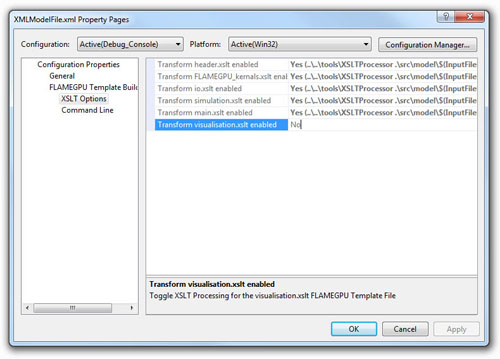
\includegraphics[width=0.70\textwidth]{img/figure2}
    \caption{FLAME GPU Build Rule XSLT Options Tab}
    \label{fig:build-rule-xslt-options-tab}
\end{figure} 

\subsection{Visual Studio Launch Configuration Command Arguments}
\label{sec:445}


In order to set the execution arguments (described in the next section) for simulation executable in any one of one of the four launch configurations, the ``Command Arguments'' property can be set form the Project Properties Page (Select ``Project'' Menu followed by ``FLAMEGPU\_Project Properties'').
The ``Command Arguments'' property is located under ``Configuration Properties -> Debug'' (see \cref{ch:3}).
Each configuration has its own set of ``Command Arguments'' so when moving between configurations these will need to be set.
Likewise the ``Configuration Properties'' are computer and user specific so these cannot be preset and must be specified the first time each example is compiled and run.
The Visual Studio macro \$InputDir can be used to specify the working directory of the project file which makes locating initial agent data XML files for many of the examples much easier (these are normally located in the iterations folders of each example).
Once a 
The Command Arguments have been set the simulation executable can be launched by selecting ``Start Debugging'' from the ``Debug'' menu or using the F5 hotkey (this is the same in both release and debug launch configurations).

\begin{figure}[ht]
    \centering
    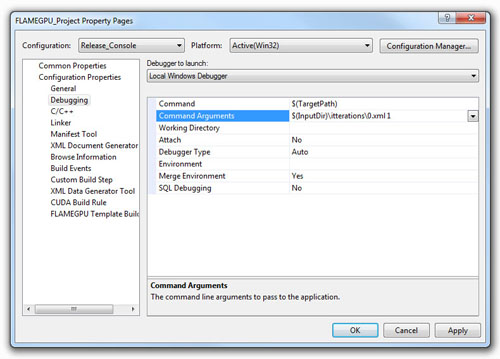
\includegraphics[width=0.70\textwidth]{img/figure3}
    \caption{FLAME GPU Project Properties Page}
    \label{fig:project-properties-page}
\end{figure} 

\section{Compilation using Make}
\label{sec:compilation-makefile}

\textbf{@todo}

\section{Simulation Execution Modes and Options}
\label{sec:45}


FLAME GPU simulations require a number of arguments depending on either console or visualisation mode. Both are described in the following subsections.


\subsection{Console Mode}
\label{sec:451}


Simulation executables built for console execution require two arguments (usage shown below).
The first of which is a file location for an initial agent XML file containing the initial agent data.
The second argument is the number of simulation iterations which should be processed.
A number of optional CUDA arguments may also be passed (i.e.
device=1 to specify the second CUDA enabled GPU device within the host machine should be used for simulation) if required.

\begin{minted}[fontsize=\small,breaklines]{text}
FLAMEGPU\_simulation.exe {[}XML model data{]} {[}Iterations{]} {[}Optional CUDA arguments{]}
\end{minted}

The result of running the simulation will be a number of output XML files which will be numbered from 1 to n, where n is the number of simulations specified by the iterations argument.
It is possible to turn XML output on or off by changing the definition of the OUTPUT\_TO\_XML macro located within the main.xslt template to true (1) false (0).

\subsection{Visualisation Mode}
\label{sec:452}

Simulation executables built for visualisation require only a single argument (usage shown below) which is the same as the first argument for with console execution (an initial agent XML file).
The number of simulations iterations is not required as the simulation will run indefinitely until the visualisation is closed.
As with console execution it is possible to specify optional CUDA arguments.

\begin{minted}[fontsize=\small,breaklines]{text}
Usage: main {[}XML model data{]} {[}Optional CUDA arguments{]}
\end{minted}

Many of the options for the default visualisation are contained within the visualisation.h header file and include the following;

\begin{itemize}
    \item \mintinline[fontsize=\small]{text}{SIMULATION_DELAY} -- Many simulations are executed extremely quickly making visualisation a blur.
        This definition allows an artificial delay by executing this number of visualisation draw loops before each simulation iteration is processed.
    \item \mintinline[fontsize=\small]{text}{WINDOW_WIDTH} and \mintinline[fontsize=\small]{text}{WINDOW_HEIGHT} -- Specifies the size of the visualisation window 
    \item \mintinline[fontsize=\small]{text}{NEAR_CLIP} and \mintinline[fontsize=\small]{text}{FAR_CLIP} -- Specifies the near an far clipping plane used for OpenGL rendering.
    \item \mintinline[fontsize=\small]{text}{SPHERE_SLICES} -- The number of slices used to create the sphere geometry representing a single agent in the visualisation.
    \item \mintinline[fontsize=\small]{text}{SPHERE_STACKS} - The number of stacks used to create the sphere geometry representing a single agent in the visualisation.
    \item \mintinline[fontsize=\small]{text}{SPHERE_RADIUS} -- The physical size of the sphere geometry representing a single agent in the visualisation.
        This will need to be a sensible value which corresponds with the environment size and agent locations within your model/simulation.
    \item \mintinline[fontsize=\small]{text}{VIEW_DISTANCE} -- The camera viewing distance.
        Again this will need to be a sensible value which corresponds with the environment size and agent locations within your model/simulation.
    \item \mintinline[fontsize=\small]{text}{LIGHT_POSITION} -- The visualisation will contain a single light source which will be located at this position.
\end{itemize}


\section{Creating a Custom Visualisation}
\label{sec:46}


Customised visualisation can easily be integrated to a FLAME GPU project by extending the automatically generated visualisation file (the output of processing visualisation.xslt)
\footnote{When doing this within Visual Studio it is important to turn off the template processing of the \mintinline[fontsize=\small]{text}{visualisation.xslt} file in each of the launch configurations as processing them will overwrite any custom code!}.
Many of the FLAME GPU SDK examples use customised visualisations in this way.
As with the default visualisations any custom visualisation must define the following function prototypes defined in the automatically generated simulation header.

\begin{minted}[fontsize=\small,breaklines]{c}
extern "C" void initVisualisation();

extern "C" void runVisualisation();
\end{minted}

The first of these can be used to initialisate any OpenGL memory and CUDA OpengGL bindings as well as displaying the user interface.
The second of these functions must take control of the simulation by repeatedly calling the draw and singleIteration (which advances the simulation by a single iteration step) functions in a recursive loop.
A more detailed description of the default rendering technique is provided within other FLAME GPU documentation (listed in \Cref{sec:12}).

\section{Performance Tips}
\label{sec:47}


The GPU offers some enormous performance advantages for agent simulation over more traditional CPU based alternatives.
With this in mind it is possible to write extremely sub optimal code which will reduce performance.
The following is a list of performance tips for creating FLAME GPU model files;

General Usage of FLAME GPU
\begin{itemize}
    \item FLAME GPU is optimal where there are very large numbers of relatively simple agents which can be parallelised.
    \item Populations of agents with very low numbers will perform poorly (in extreme cases slower than if they were simulated using the CPU).
        If you require an agent population with very few agents consider writing some custom CPU simulation code and transferring any important information into simulation constants to be read by larger agent populations during the FLAME GPU simulation step.
    \item Outputting information to disk (XML files) is painfully slow in comparison with simulation speeds so consider outputting information visually or only after larger numbers of simulation iterations.
\end{itemize}

Model Specification

\begin{itemize}
    \item Minimise the number of variables with agents and message data where possible.
    \item Try to conceptualise and fully specify the model before completing the agent functions script to avoid making mistakes with agent function arguments.
        Try to think in terms of X-Machines agents!
\end{itemize}

Agent Function Scripting

\begin{itemize}
    \item Small compute intensive agent functions are more efficient than functions which only iterate messages.
        Try to minimise the number of times message lists are iterated.
    \item Keep agent functions small and do not define more local variables than is strictly required.
        Reuse local variables where possible if they are no longer needed and before they go out of scope.
\end{itemize}

Message Iteration

\begin{itemize}
    \item For small populations of agents (generally less than 2000 but dependant on hardware and the model) non partitioned messaging has less overhead and is similarly comparable to spatial partitioning.
    \item For large populations of distributed agents with limited communication spatially partitioned message communication will be much faster.
\end{itemize}

% \bibliography{bib/bib}

\end{document}
